\chapter{\label{cha:sts_sentence_encoders}Exploring STS with Sentence Encoders}

\section{Introduction}
The main goal of a sentence encoder is to map a variable-length text to a fixed-length vector representation. In basic terms, a sentence encoder would take a sentence or text as the input and would output a vector. This vector encodes the meaning of the sentence and can be used for downstream tasks such as text classification, text similarity etc. In these down stream tasks, the sentence encoder is often considered as a black box where the users use the sentence encoder to get sentence embeddings without knowing what exactly happens in the encoder itself. 

Ideally, the approaches we experimented in Chapter \ref{cha:sts_state_of_the_art_methods} like Vector Averaging, Smooth Inverse Frequency \cite{DBLP:conf/iclr/AroraLM17} can also be considered as sentence encoders since in those approaches the input is a variable-length text and the output is a fixed-length vector. However, these approaches have major drawbacks in representing sentences. One such drawback is these approaches do not care about the word order. If you consider two sentences \textit{"Food is good but the service is bad"} and \textit{"Food is bad but the service is good"}, would have the same embeddings from these approaches even though the meaning of these two sentences is completely different. Another drawback is those approaches lose information in the vector aggregation process. If you consider two sentences \textit{"It is great"} and \textit{"It is not great"}, Vector Averaging and Smooth Inverse Frequency would give similar sentence embeddings as there is only one word difference in the two sentences. Even though this affect can be minimised using techniques like TF/IDF weighting that we explored in Chapter \ref{cha:sts_state_of_the_art_methods}, a different approach would be to train end-to-end models to get sentence embeddings. These models are commonly addressed as \textit{sentence encoders} in NLP community.

Over the years, various sentence encodes like Sent2vec \cite{pagliardini-etal-2018-unsupervised}, Infersent  \cite{cer2018universal}, Universal Sentence Encoder \cite{conneau-EtAl:2017:EMNLP2017} have been proposed. Even though most of these sentence encoders have sophisticated architectures, since many are using them only as a black box to get the sentence embeddings, they have been very popular in the NLP community. As the sentence encoders provide good quality sentence embeddings efficiently, the word embedding aggregation methods like Vector Averaging, Smooth Inverse Frequency have been often overlooked by the community in favour of sentence encoders. 

Once you have the sentence embedding from a sentence encoder, using them to calculate STS is an easy task. Since these sentence embeddings are already semantically powerful, a simple vector comparison technique like cosine similarity between the embeddings can be used to calculate the STS of the two sentences. Therefore, pre-trained sentence encoders can be used as an unsupervised STS method. However, even though the sentence encoders have been commonly used in STS tasks, there is no comprehensive study done on them. Since most of the researchers are using sentence encoders as a black box in many applications, they don't understand the limitations of using them. In this chapter we are addressing this gap by exploring sentence encoders in different STS datasets adopting them in different languages and domains. With a study like this we can understand the limitations of the sentence encoders and when not to use them. 

We address three research questions in this chapter:

\textbf{RQ1:} How well the sentence encoders perform in English STS datasets?

\textbf{RQ2:} Can the sentence encoders be easily adopted in different languages?

\textbf{RQ3:} How well the sentence encoders perform in different domains?

The main contributions of this chapter are as follows.

\begin{enumerate}
	\item In the Related Work Section (Section \ref{sec:sentence_related}), we discuss three sentence encoders that are popular in the NLP community. 
	
	\item  We evaluate these three sentence encoders on three English STS datasets, two non-English STS datasets and a bio-medical STS dataset which were introduced in Chapter \ref{cha:sts_introduction}.
	
	\item The code with the experiments conducted are publicly available to the community\footnote{The public GitHub repository is available on \url{https://github.com/tharindudr/simple-sentence-similarity}}.
	
\end{enumerate}

The rest of this chapter is organised as follows. Section \ref{sec:sentence_related} describes the three sentence encoders we experimented in this section. In Section \ref{sec:sentence_method} we present the experiments we conducted with the three sentence encoders in English STS datasets followed by the results comparing with the other unsupervised STS methods. Section \ref{sec:sentence_languages} and Section \ref{sec:sentence_domains} shows how sentence encoders can be applied to different languages and domains and their results. The chapter finishes with conclusions and ideas for future research directions in sentence encoders.


\section{Related Work}
\label{sec:sentence_related}
As we mentioned before, the sentence encoders are popular with the NLP community. The three sentence encoders explored in this chapter: Sent2vec \cite{pagliardini-etal-2018-unsupervised}, Infersent \cite{conneau-EtAl:2017:EMNLP2017} and Universal Sentence Encoder \cite{cer2018universal} are the most common sentence encoders. Other than them there is also Doc2vec \cite{pmlr-v32-le14} which is can be considered as a sentence encoder. However, due to the various upgrades in different python libraries, the official pre-trained Doc2vec models are not working any more. Therefore, we only used following sentence encoders in our experiments.

\paragraph{Sent2vec}
Sent2vec presents a simple but efficient unsupervised objective to train distributed representations of sentences \cite{pagliardini-etal-2018-unsupervised}. It can be thought as an extension of Word2vec (CBOW) to sentences. The key differences between CBOW and Sent2Vec are the removal of the input subsampling, considering the entire sentence as context, as well as the addition of word n-grams. With Sent2vec, sentence embedding is defined as the average of the word embeddings of its constituent words. The objective of Sent2vec is similar to CBOW; predict the missing word given the context \cite{pagliardini-etal-2018-unsupervised}. 

Sent2vec has officially released several pre-trained models to derive the sentence embeddings\footnote{The code and the pre-trained models are available on \url{https://github.com/epfml/sent2vec}}. Also due to its unsupervised approach and simple objective function, Sent2vec has been adopted in different languages and domains too.  


\paragraph{Infersent}
InferSent is an NLP technique for universal sentence representation developed by Facebook which uses supervised training to produce high quality sentence vectors \cite{conneau-EtAl:2017:EMNLP2017}. The authors explore 7 different architectures for sentence
encoding including LSTM \cite{10.1162/neco.1997.9.8.1735}, GRU \cite{Chung2014EmpiricalEO}, Bi directional LSTM \cite{650093} with mean/max pooling, Self-attentive network and Hierarchical Deep Convolutional Neural Network \cite{conneau-EtAl:2017:EMNLP2017}. All of these models were trained for the natural language inference (textual entailment) task using the architecture in Figure \ref{fig:infersent_general}. They evaluate the quality of the sentence representation by using them as features in 12 different transfer tasks like Binary and multi-class text classification, semantic textual similarity, paraphrase detection etc. The results indicate that the BiLSTM with the max-pooling operation performs best on these tasks  \cite{conneau-EtAl:2017:EMNLP2017}. The architecture of this BiLSTM with the max-pooling model is shown in Figure \ref{fig:infersent_architecture}.

Facebook released two models to derive the sentence embeddings. One model is trained with GloVe \cite{pennington-etal-2014-glove} which in turn has been trained on text preprocessed with the PTB tokeniser and the other model is trained with fastText \cite{mikolov-etal-2018-advances}  which has been trained on text preprocessed with the MOSES tokeniser. We used both models in our experiments\footnote{The code and the pre-trained models are available on \url{https://github.com/facebookresearch/InferSent}}.



\begin{figure}
	\captionsetup[subfigure]{justification=centering}
	\centering
	\begin{subfigure}[b]{.5\textwidth}
		\centering
		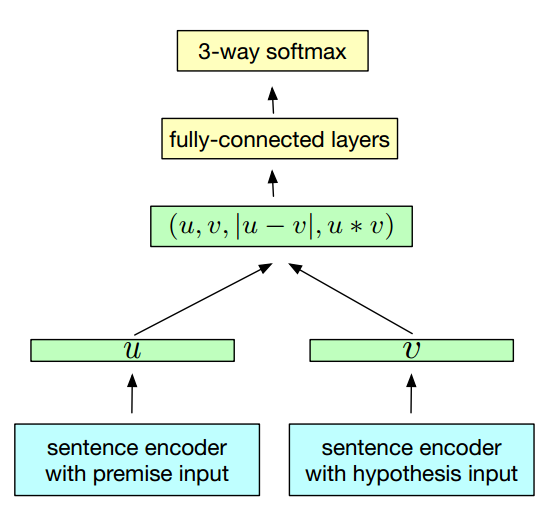
\includegraphics[width=\textwidth]{figures/semantic_textual_similarity/sentence_encoders/infersent_general.png}
		\caption{General NLI Training Scheme.}
		\label{fig:infersent_general}
	\end{subfigure}%
	\begin{subfigure}[b]{.5\textwidth}
		\centering
		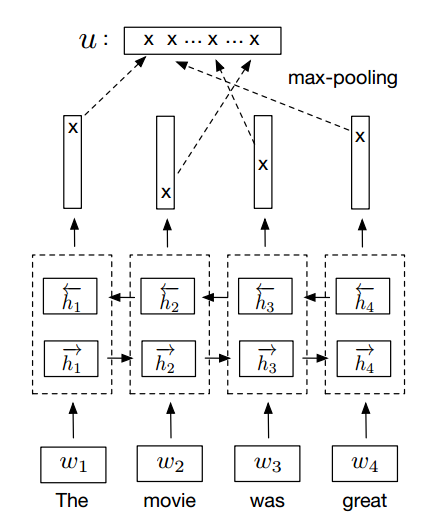
\includegraphics[width=\textwidth]{figures/semantic_textual_similarity/sentence_encoders/infersent.png}
		\caption{Bi directional LSTM  with max pooling}
		\label{fig:infersent_architecture}
	\end{subfigure}
	\caption[Infersent Architecture]{General NLI training scheme in Infersent with the best architecture; Bi directional LSTM  with max pooling \cite{conneau-EtAl:2017:EMNLP2017}. }
	\label{fig:infersent}
\end{figure}

\paragraph{Universal Sentence Encoder}

The Universal Sentence Encoder \cite{cer2018universal} released by Google is the last sentence encoder we employed in this chapter. This is again an unsupervised sentence encoder. It comes with two versions i.e. one trained with Transformer encoder and other trained with Deep Averaging Network
(DAN). Both architectures are outlined briefly below. The two have a trade-off of accuracy and computational resource requirement. While the one with Transformer encoder has higher accuracy, it is computationally more expensive. The one with DAN encoding is computationally less expensive but with slightly lower accuracy.

The original Transformer encoder model constitutes an encoder and decoder. Since our research is only focussed on encoding sentences to vectors, we only use its encoder part. The encoder is composed of a stack of N = 6 identical layers. Each layer has two sub-layers. The first is a multi-head self-attention mechanism, and the second is a simple, position-wise fully connected feed-forward network. \citet{cer2018universal} also employed a residual connection around each of the two sub-layers,
followed by layer normalisation. Since the model contains no recurrence and no convolution, for the model to make use of the order of the sequence, it must inject some information about the relative or absolute position of the tokens in the sequence, that is what the “positional encodings” does. The transformer-based encoder achieves the best overall transfer task performance. However, this comes at the cost of computing time and memory usage scaling dramatically with sentence length.

Deep Averaging Network (DAN) is much simpler where input embeddings for words and bi-grams are first averaged together and then passed through a feedforward deep neural network to produce sentence embeddings. The primary advantage of the DAN encoder is that computation time is linear in the length of the input sequence. With this sentence encoder too, we used both architectures in our experiments\footnote{Pre-trained sentence encoder for transformer model is available on \url{https://tfhub.dev/google/universal-sentence-encoder-large} and pre-trained sentence encoder for DAN model is available on \url{https://tfhub.dev/google/universal-sentence-encoder}.} Unlike the other sentence encoders, Google officially released two multilingual models for Universal Sentence Encoder.

\begin{figure}
	\captionsetup[subfigure]{justification=centering}
	\centering
	\begin{subfigure}[b]{.35\textwidth}
		\centering
		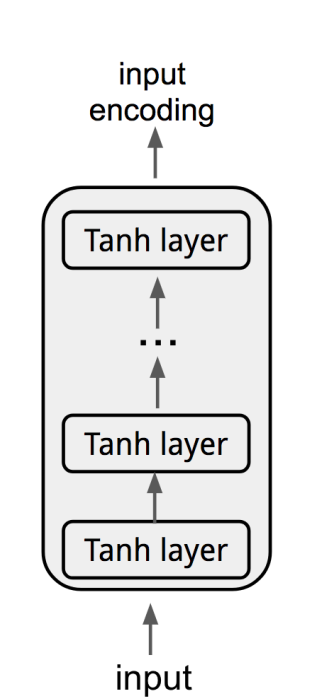
\includegraphics[width=\textwidth]{figures/semantic_textual_similarity/sentence_encoders/dan.png}
		\caption{DAN Architecture}
		\label{fig:dan}
	\end{subfigure}%
	\begin{subfigure}[b]{.35\textwidth}
		\centering
		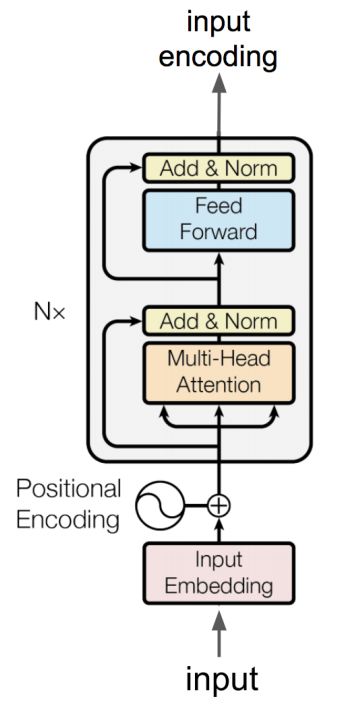
\includegraphics[width=\textwidth]{figures/semantic_textual_similarity/sentence_encoders/transformer.png}
		\caption{Transformer Architecture}
		\label{fig:transformer}
	\end{subfigure}
	\caption[Universal Sentence Encoder Architectures]{Two architectures in Universal Sentence Encoders.}
	\label{fig:use}
\end{figure}

\section{Exploring Sentence Encoders in English STS}
\label{sec:sentence_method}
Adopting sentence encoders for STS is an easy task.  If two embeddings from the two sentences are closer, the sentences are said to be semantically similar. As the approach, first the two sentences are passed to the sentence encoders to get the embeddings and the we calculate the cosine similarity between the resulting embeddings which represents the textual similarity of the two input sentences. To be clear, if the two vectors for two sentences X and Y are $a$ and $b$ correspondingly, we calculate the cosine similarity between $a$ and $b$ as of equation \ref{equ:cosine} and use that value to represent the similarity between the two sentences. 

\begin{equation}
	\label{equ:cosine}
	\begin{aligned}
		\cos ({\bf a},{\bf b})= {} & {{\bf a} {\bf b} \over \|{\bf a}\| \|{\bf b}\|} \\
		= {} & \frac{ \sum_{i=1}^{n}{{\bf a}_i{\bf b}_i} }{ \sqrt{\sum_{i=1}^{n}{({\bf a}_i)^2}} \sqrt{\sum_{i=1}^{n}{({\bf b}_i)^2}} }
	\end{aligned}
\end{equation}

First we experimented with English STS datasets we explained in Section \ref{sec:sts_intro_datsets}. For the experiments we used all the sentence encoders mentioned in Section \ref{sec:sentence_related}. For \textbf{Sent2vec}, we used the pre-trained Sent2vec model, \textit{sent2vec\_wiki\_bigrams} trained on English Wikipedia articles. Using that we could represent a sentence from a 700 dimensional vector. For \textbf{Infersent}, as we mentioned before, there are two pre-trained models available; \textit{infersent1} which was trained using GloVe \cite{pennington-etal-2014-glove} and \textit{infersent2} which was trained using fastText \cite{mikolov-etal-2018-advances}. Both models have been trained on the SNLI dataset which consists of 570k human generated English sentence pairs, manually labelled with one of the three categories: entailment, contradiction and neutral \cite{bowman-etal-2015-large}. Using that we could represent a sentence from a 512 dimensional vector. For \textbf{Universal Sentence Encoder}, we used universal-sentence-encoder (DAN architecture) and universal-sentence-encoder-large (Transformer architecture) which were trained on text resources like Wikipedia and news articles. With that too we could represent a sentence from a 512 dimensional vector.

We evaluated these three sentence encoders in three English STS datasets that we explained in Section \ref{sec:sts_intro_datsets}; SICK, STS2017 and QUORA.  Table \ref{tab:sick_sentence_encoder} shows the results for SICK dataset, Table \ref{tab:sts_sentence_encoder} shows the results for STS 2017 dataset and Table \ref{tab:quora_sentence_encoder} shows the results for Quora Questions Pairs dataset.


\begin{table*}[htb]
	%\footnotesize
	\centering
	\scalebox{0.95}{
		\begin{tabular}{|l|cc|}
			\hline
			\textbf{Model} & $\bm{\rho}$   & $\bm{\tau}$     
			\\ \hline
			\textit{ELMo $\bigoplus$ BERT}                     
			& 0.753  & 0.669       \\
			\hline
			\textit{Sent2vec}                     
			& 0.759  & 0.672      \\
			\hline
			\textit{Infersent1}                     
			& 0.763  & 0.679      \\\hline
			\textit{Infersent2}                     
			& 0.769  & 0.684      \\\hline
			\textit{USE (DAN)}                     
			& 0.772  & 0.695     \\\hline
			\textit{USE (Transformer)}                     
			& 0.780$^{\dagger}$  & 0.721$^{\dagger}$       \\
			
			\hline
		\end{tabular}
	}
	\caption[Results for SICK with sentence encoders]{Results for SICK dataset with sentence encoders. For each sentence encoder, Pearson Correlation ($\bm{\rho}$) and Spearman Correlation ($\bm{\tau}$) are reported between the predicted values and the gold labels of the test set. USE denotes Universal Sentence Encoder. Additionally, we report the results of the best model from Chapter \ref{cha:sts_state_of_the_art_methods}; \textit{ELMo $\bigoplus$ BERT}. Best result from all the methods is marked with ${\dagger}$. }  
	\label{tab:sick_sentence_encoder}
\end{table*}


\begin{table*}[htb]
	%\footnotesize
	\centering
	\scalebox{0.95}{
		\begin{tabular}{|l|cc|}
			\hline
			\textbf{Model} & $\bm{\rho}$   & $\bm{\tau}$     
			\\ \hline
			\textit{ELMo $\bigoplus$ BERT}                     
			& 0.654  & 0.616      \\
			\hline
			\textit{Sent2vec}                     
			& 0.673  & 0.645       \\
			\hline
			\textit{Infersent1}                     
			& 0.703  & 0.696       \\
			\hline
			\textit{Infersent2}                     
			& 0.711  & 0.701       \\
			\hline
			\textit{USE(DAN)}                     
			& 0.725  & 0.703       \\
			\hline
			\textit{USE(Transformer)}                     
			& 0.744$^{\dagger}$  & 0.721$^{\dagger}$       \\
			\hline
		\end{tabular}
	}
	\caption[Results for STS 2017 with sentence encoders]{Results for STS 2017 dataset with sentence encoders. For each sentence encoder, Pearson Correlation ($\bm{\rho}$) and Spearman Correlation ($\bm{\tau}$) are reported between the predicted values and the gold labels of the test set. USE denotes Universal Sentence Encoder. Additionally, we report the results of the best model from Chapter \ref{cha:sts_state_of_the_art_methods}; \textit{ELMo $\bigoplus$ BERT}. Best result from all the methods is marked with ${\dagger}$. }  
	\label{tab:sts_sentence_encoder}
\end{table*}


\begin{table*}[htb]
	%\footnotesize
	\centering
	\scalebox{0.95}{
		\begin{tabular}{|l|c|}
			\hline
			\textbf{Model} & RMSE     
			\\ \hline
			\textit{ELMo $\bigoplus$ BERT}                     
			& 0.566    \\
			\hline
			\textit{Sent2vec}                     
			& 0.632   \\
			\hline
			\textit{Infersent1}                     
			& 0.642    \\
			\hline
			\textit{Infersent2}                     
			& 0.653    \\
			\hline
			\textit{USE(DAN)}                     
			& 0.666    \\
			\hline
			\textit{USE(Transformer)}                     
			& 0.686$^{\dagger}$    \\
			
			\hline
		\end{tabular}
	}
	\caption[Results for QUORA with sentence encoders]{Results for QUORA dataset with sentence encoders. For each sentence encoder model, Root Mean Squared Error (RMSE) is reported. USE denotes Universal Sentence Encoder. Additionally, we report the results of the best model from Chapter \ref{cha:sts_state_of_the_art_methods}; \textit{ELMo $\bigoplus$ BERT}. Best result is marked with ${\dagger}$.}  
	\label{tab:quora_sentence_encoder}
\end{table*}

As can be seen in the results, Universal Sentence Encoder outperformed all other sentence encoders in all the English STS datasets. From the two architectures available in the Universal Sentence Encoder, Transformer architecture outperforms the DAN architecture as they have explained in their paper. Furthermore, it should be noted that in all three datasets, sentence encoders outperform the embedding aggregation based smooth inverse frequency method that performed best in Chapter \ref{cha:sts_state_of_the_art_methods}. This concludes that sentence encoders generally perform better than embedding aggregation techniques in STS. 

With these results, we can answer our \textbf{RQ1}, sentence encoders can be easily adopted and perform well in English STS tasks. However, most of these models are complex in nature which would result in more processing time/resources which can be chaotic in some situations. 


\section{Portability to Other Languages}
\label{sec:sentence_languages}
Our \textbf{RQ2} targets the multilinguality aspect of the sentence encoders; \textit{How well the sentence encoders perform in different languages?}. To answer this, we evaluated our method in Arabic STS and Spanish STS datasets that were introduced in Chapter \ref{cha:sts_introduction}. With these experiments, we identified a main weakness in sentence encoders; sentence encoders pre-trained on different languages are not easy to find. 

If you consider \textbf{Infersent}, it was pre-trained using the SNLI dataset which consists of 570k human generated English sentence pairs, manually labelled with one of three categories: entailment, contradiction and neutral \cite{bowman-etal-2015-large}. If someone is adopting \textbf{Infersent} for a different language other than English, they need to have a corpus similar to SNLI with a similar size. Annotating such a corpus for a different language would be challenging. Even though there are some attempts like XNLI \cite{conneau-etal-2018-xnli} to create such a corpus, the number of annotated instances are very limited. This makes it difficult to adopt \textbf{Infersent} in other languages which is a clear limitation of the Infersent architecture. 

However, the other two sentence encoders we experimented in this Chapter; Sent2vec and Universal Sentence Encoder are in a better position in multilingualism compared to Infersent as they don't require a large annotated corpus like SNLI. Both of those sentence encoders have been trained on unsupervised textual data which will be easy to find in most of the languages. However, still they need powerful computing resources to train the models which is a challenge when adopting these sentence encoders to different languages. 

For \textbf{Sent2Vec}, there was no Arabic pre-trained model available. However, there is a Spanish Sent2vec model\footnote{The pre-trained model is available on \url{https://github.com/BotCenter/spanish-sent2vec}} available which is pre-trained on Spanish Unannotated Corpora. Using that we could represent a Spanish sentence with a 700 dimensional vector. For \textbf{Universal Sentence Encoder}, there is a multilingual version which supports 16 languages\footnote{The model currently supports Arabic, Chinese-simplified, Chinese-traditional, English, French, German, Italian, Japanese, Korean, Dutch, Polish, Portuguese, Spanish, Thai, Turkish and Russian.} including Arabic and Spanish \cite{yang-etal-2020-multilingual}. This multilingual model is available in both architecture in Universal Sentence Encoder; DAN and Transformer\footnote{The multilingual Universal Sentence Encoder with DAN architecture is available on \url{https://tfhub.dev/google/universal-sentence-encoder-multilingual/3} and the multilingual Universal Sentence Encoder with Transformer architecture is available on \url{https://tfhub.dev/google/universal-sentence-encoder-multilingual-large/3}.}. Using that we could represent the Arabic and Spanish sentences with a 512 dimensional vector. As we mentioned before, for \textbf{Infersent}, we could not find any pre-trained models that supports either Arabic nor Spanish. Therefore, we did not use Infersent in our multilingual experiments. The Arabic and Spanish STS results with the mentioned sentence encoders are available in Table \ref{tab:arabic_spanish_sentence_encoder}.

\begin{table*}[htb]
	%\footnotesize
	\centering
	\scalebox{0.95}{
		\begin{tabular}{|c|c|c|c|}
			\hline
			\textbf{Language} &	\textbf{Sentence Encoder} &  $\bm{\rho}$ & $\bm{\tau}$     
			\\ \hline
			\multirow{ 3}{*}{\textit{Arabic}}	& \textit{ELMo $\bigoplus$ BERT}                    
			& 0.624 & 0.589 \\
			&	\textit{USE (DAN)}                     
			& 0.654 & 0.612 \\
			&	\textit{USE (Transformer)}                     
			& 0.668$^{\dagger}$ & 0.635$^{\dagger}$ \\
			\hline
				\multirow{ 4}{*}{\textit{Spanish}}	& \textit{ELMo $\bigoplus$ BERT}                    
			&  0.712 & 0.663\\
			&	\textit{USE (DAN)}                     
			& 0.723 & 0.6.682 \\
			& \textit{Sent2vec} & 0.725 & 0.688 \\
			&	\textit{USE (Transformer)}                     
			& 0.741$^{\dagger}$ & 0.702$^{\dagger}$ \\
			\hline
		\end{tabular}
	}
	\caption[Results for Arabic and Spanish STS with Sentence Encoders]{Results for Arabic and Spanish STS with different sentence encoders. For each sentence encoder, Pearson Correlation ($\bm{\rho}$) and Spearman Correlation ($\bm{\tau}$) are reported between the predicted values and the gold labels of the test set. USE denotes Universal Sentence Encoder. Additionally, we report the results of the best model from Chapter \ref{cha:sts_state_of_the_art_methods}; \textit{ELMo $\bigoplus$ BERT}. Best result for each language is marked with ${\dagger}$.}  
	\label{tab:arabic_spanish_sentence_encoder}
\end{table*}

As can be seen in results, similar to the English datasets, from the sentence encoders we considered,  Universal Sentence Encoder with the Transformer architecture gave the best results for both Arabic and Spanish datasets. From the two architectures available in the Universal Sentence Encoder, Transformer architecture outperforms the DAN architecture in both languages. Furthermore, it should be noted that in both languages, sentence encoders outperform the word embedding based smooth inverse frequency method that performed best in Chapter \ref{cha:sts_state_of_the_art_methods}.  

With these experiments, we can answer our \textbf{RQ2: How well the sentence encoders can be adopted in different languages?}. Adopting sentence encoders in different languages is challenging since there are no available pre-trained sentence encoder models for many languages. However, in the cases where they are available, it is very easy to use them in STS tasks and they provide good results compared to other unsupervised STS methods. 


\section{Portability to Other Domains}
\label{sec:sentence_domains}

In order to answer our \textit{RQ3}; how well the sentence encoders can be applied in different domains, we evaluated sentence encoders that we explained in this Chapter on the Bio-medical STS dataset explained in \ref{cha:sts_introduction}. As we mentioned before, Bio-medical STS dataset does not have a training set. Therefore, only the unsupervised approaches can be applied on this dataset which provides an ideal opportunity for the sentence encoders we experimented in this chapter. 

However, we faced the same issue we faced in Arabic and Spanish STS experiments in Bio-medical STS experiments too. There are not many options when it comes to sentence encoders that were trained on Bio-medical domain \cite{TAWFIK2020103396}. For \textbf{Sent2vec}, we could find a pre-trained model in Bio-medical domain which was trained using PubMed data \cite{8904728}\footnote{The code and the pre-trained model is available on \url{https://github.com/ncbi-nlp/BioSentVec}}. However, for other two sentence encoders, we could not find any available pre-trained sentence encoder models on Bio-medical domain. Therefore, for Universal Sentence Encoder and Infersent, we had to use pre-trained sentence encoder models trained on English texts for this experiments. The results are shown in Table \ref{tab:biosses_sentence_encoders}.

\begin{table*}[htb]
	%\footnotesize
	\centering
	\scalebox{0.95}{
		\begin{tabular}{|l|c|}
			\hline
			\textbf{Model} & $\bm{\rho}$   \\  
			\hline
			\textit{Infersent2} & 0.294 \\
			\textit{Infersent1} & 0.301 \\
			\textit{USE(DAN)} & o.321 \\
			\textit{USE(Transformer)} & 0.345 \\
			\textit{ELMo $\bigoplus$ BERT}  &  0.708 \\
			\textit{BioSentVec} \cite{8904728} & 0.810$^{\dagger}$  \\
			\hline
		\end{tabular}
	}
	\caption[Results comparison for BIOSSES with different sentence encoders]{Results for BIOSSES dataset with different sentence encoders compared with top results reported for BIOSSES. Additionally, we report the results of the best model from Chapter \ref{cha:sts_state_of_the_art_methods}; \textit{ELMo $\bigoplus$ BERT}. For each variant, Pearson Correlation ($\bm{\rho}$) is reported between the predicted values and the gold labels of the test set. Best result is marked with ${\dagger}$.}  
	\label{tab:biosses_sentence_encoders}
\end{table*} 

As can be observed in the results, sentence encoder trained on the Bio-medical domain; BioSentVec \cite{8904728} outperformed other approaches. In fact, when compared to the best results in the BIOSSES dataset BioSentVec outperforms all of them which means that BioSentVec provides the best result for BIOSSES. it should be noted that out of domain sentence encoders like Universal Sentence Encoder and Infersent, that were not trained on the Bio-medical domain performed very poorly in these experiments. The simple \textit{ELMo $\bigoplus$ BERT} embedding aggregation based approach we experimented in Chapter \ref{cha:sts_state_of_the_art_methods} outperforms Universal Sentence Encoder and Infersent by a large margin. This can be due to the fact that, there is a large number of out-of-vocabulary words for these general sentence coders in the Bio-medical domain unlike the \textit{ELMo $\bigoplus$ BERT} where we used the ELMo and BERT models trained on Bio-medical domain. We can conclude that sentence encoders can be successfully adopted for STS in different domains, however they won't succeed unless they are pre-trained on that particular domain. 

With these finding we answer our \textbf{RQ3: Is it possible to adopt sentence encoders in different domains?}. We showed that it is possible to adopt sentence encoders in a different domain. However, it is difficult since pre-trained sentence encoder models are not common in most domains and the sentence encoders pre-trained on a general domain perform poorly on a specific domain like Bio-medical. 

\section{Conclusions}
\label{sec:sentence_conclusions}
In this chapter we experimented another unsupervised STS method; sentence encoders. We explored three popular sentence encoders; Sent2vec, Infersent and Universal Sentence Encoder in three English STS datasets. The results show that sentence encoders outperforms other unsupervised STS methods. From the sentence encoders, Universal Sentence Encoder with the Transformer architecture performs best in all three datasets. Furthermore, we evaluated sentence encoders in different languages and domains. We experienced the biggest hurdle in adopting sentence encoders in different languages and domains; the pre-trained sentence encoders that support different languages and domains are not common compared to the word embedding/ contextual word embedding models available on those languages and domains. This is because the sentence encoders take a lot of time to train and some of the sentence encoders like Infersent require specific training data, which is hard to compile in most of the languages and domains. Also, since the applications of sentence encoders are limited compared to word embeddings/ contextual word embeddings people have not spend time on creating language specific and domain specific sentence encoders. However, when available they perform very well in the relevant tasks. Also we tried to use sentence encoders that were trained on a general domain in a different but specific domain like Bio-medical. This provided very poor results. Therefore, we can conclude that using sentence encoders on a different domain to their pre-trained domain won't provide good results.


Being an unsupervised STS method, the sentence encoders have the obvious advantage of not needing a training set for STS. However, they still need a pre-trained sentence encoding model, which is not available in most of the languages and domains. This is a major drawback in sentence encoders compared to the embedding aggregation methods since the word embedding/ contextual embedding models are commonly available in many languages and domains. This is worsened by the fact that sentence encoders perform very poorly on the domains that they did not see in the training process. This suggests that we should only use sentence encoders when available in a certain domain/ language, otherwise using embedding aggregation methods like Smooth Inverse Frequency would provide better results. 


As future work, the experiments can be extended in to recently released sentence encoders like LASER \cite{10.1162/tacl_a_00288}. LASER supports 93 languages including low resource languages like Kabyle, Malagasy, Sinhala etc. This should solve some of the multilingual issues we experienced with sentence encoders in this chapter. Very recently sentence encoders have been explored with Siamese neural architectures and  Transformers. We discuss them in Chapters \ref{cha:sts_siamese_neural_networks} and \ref{cha:sts_transformers}. 
